\documentclass[12pt,a4paper]{article}

% Impostazioni di base del documento
\usepackage[T1]{fontenc}
\usepackage[utf8]{inputenc}
\usepackage[italian]{babel}
\usepackage[a4paper,margin=2cm]{geometry}
\usepackage{microtype}
\usepackage{graphicx}
\usepackage{amsmath}
\usepackage{booktabs}
\usepackage[hidelinks]{hyperref}

\setlength{\parindent}{0pt}
\setlength{\parskip}{0.5em}

% Informazioni del frontespizio
\newcommand{\university}{Università degli Studi di Salerno}
\newcommand{\degreecourse}{Corso di Laurea Magistrale in Ingegneria Informatica}
\newcommand{\reporttitle}{Segmentazione dei filamenti solari}
\newcommand{\teamname}{2026\_MLrec\_gr02}
\newcommand{\members}{Francesco Peluso}
\newcommand{\academicyear}{2025/2026}

\begin{document}
\pagenumbering{gobble}

\begin{titlepage}
  \centering

  {\Large \university\par}
  \vspace{0.4cm}
  {\large \degreecourse\par}

  \vfill

  {\Huge\bfseries \reporttitle\par}
  \vspace{0.5cm}
  {\Large Relazione del progetto di Machine Learning\par}

  \vfill

  {\large
    \textbf{Gruppo}\par
    \teamname\par
    \vspace{0.6cm}
    \textbf{Componenti}\par
    \members\par
  }

  \vfill

  {\large Anno accademico \academicyear\par}
\end{titlepage}

\pagenumbering{arabic}

\section{Introduzione}
\label{sec:introduction}

L'obiettivo di questo progetto è identificare i filamenti solari nelle immagini del Sole mediante tecniche di Machine Learning. Il problema è formulato come un'attività di \textbf{segmentazione semantica binaria}: data un'immagine solare, il modello deve produrre una maschera binaria in cui ogni pixel viene classificato come \textit{filamento} oppure \textit{sfondo}.

L'analisi delle immagini di addestramento evidenzia alcune difficoltà rilevanti. I filamenti solari si presentano generalmente come strutture scure, sottili e irregolari sul disco solare. Il loro contrasto rispetto alle regioni circostanti può essere basso, mentre forma e dimensioni possono variare considerevolmente tra immagini diverse. Inoltre, la superficie solare contiene altre strutture e rumore di fondo che possono avere caratteristiche visive simili a quelle di un filamento.

Un altro aspetto importante è il forte sbilanciamento tra le due classi. In genere, i filamenti occupano solo una piccola porzione dell'immagine completa, mentre la maggior parte dei pixel appartiene allo sfondo. Per questo motivo, identificare correttamente le regioni dei filamenti è più importante che massimizzare semplicemente l'accuratezza della classificazione a livello di pixel.

Il progetto si concentra quindi su modelli capaci di combinare l'estrazione di caratteristiche di alto livello con la conservazione delle informazioni spaziali fini. La qualità della segmentazione ottenuta viene valutata principalmente mediante il \textbf{coefficiente di Dice}, che misura la sovrapposizione tra la maschera binaria predetta e la corrispondente maschera di riferimento (\textit{ground truth}).

\section{Approccio proposto}
\label{sec:approach}

\subsection{Architettura della rete}

L'approccio principale considerato per questo progetto si basa su una
\textbf{rete neurale convoluzionale U-Net}, un'architettura progettata
specificamente per la segmentazione delle immagini.

Le architetture CNN studiate per la classificazione delle immagini non
sono direttamente adatte al nostro problema. Una rete di classificazione
estrae progressivamente le caratteristiche da un'immagine e produce infine
una predizione per l'intero ingresso, come un'etichetta di classe. Nella
segmentazione semantica, invece, è importante anche la posizione delle
caratteristiche rilevate, poiché la rete deve assegnare una classe a ogni
pixel dell'immagine.

U-Net affronta questo problema mediante due percorsi principali. Il primo
estrae progressivamente caratteristiche di livello più elevato e ne riduce
la risoluzione spaziale, in modo analogo a una CNN standard. Il secondo
aumenta progressivamente la risoluzione di tali caratteristiche fino a
ottenere una maschera di segmentazione.

Una caratteristica importante di U-Net è l'impiego di \textbf{connessioni
di salto} (\textit{skip connections}) tra diverse parti della rete. Queste
connessioni consentono di riutilizzare, durante la costruzione della
maschera di uscita, le caratteristiche che contengono informazioni spaziali
fini. Ciò è particolarmente utile nel nostro problema, poiché i filamenti
solari possono essere sottili, irregolari e difficili da distinguere dalla
superficie solare circostante.

\subsection{Vantaggi e limitazioni}

I principali vantaggi di questo approccio sono:

\begin{itemize}
    \item U-Net è progettata specificamente per la segmentazione delle
          immagini a livello di pixel;
    \item si basa principalmente su operazioni convoluzionali, già adatte
          all'estrazione di caratteristiche spaziali dalle immagini;
    \item le connessioni di salto aiutano a conservare le informazioni
          relative alle strutture piccole e sottili;
    \item l'architettura è relativamente semplice e può essere modificata
          per valutare sperimentalmente configurazioni diverse.
\end{itemize}

È necessario considerare anche alcune limitazioni:

\begin{itemize}
    \item la riduzione della risoluzione spaziale può causare la perdita di
          informazioni relative ai filamenti molto sottili;
    \item l'elaborazione di immagini ad alta risoluzione richiede una
          maggiore quantità di memoria della GPU;
    \item il forte sbilanciamento tra i pixel appartenenti ai filamenti e
          quelli appartenenti allo sfondo può rendere più difficile
          l'addestramento;
    \item strutture dall'aspetto simile ai filamenti possono generare
          predizioni false positive.
\end{itemize}

\subsection{Approcci alternativi}

Come alternativa, si potrebbe considerare una \textbf{U-Net residua}
(\textit{Residual U-Net}), introducendo blocchi residui e connessioni di
salto all'interno della rete. Ciò consentirebbe di analizzare, nel contesto
della segmentazione delle immagini, le tecniche di apprendimento residuo
studiate durante il corso.

Un'altra possibilità consiste nell'utilizzare una \textbf{CNN preaddestrata}
come parte dell'architettura U-Net e applicare il \textit{transfer learning}
e il \textit{fine-tuning}. Questo approccio potrebbe essere utile soprattutto
se l'insieme di addestramento disponibile non fosse sufficientemente ampio
da consentire l'apprendimento da zero di caratteristiche visive robuste.

Si potrebbero considerare anche architetture di segmentazione più avanzate.
Tuttavia, U-Net rappresenta un punto di partenza adeguato grazie alla sua
architettura relativamente semplice e all'impiego diretto di strati
convoluzionali e connessioni di salto.

\section{Criteri di valutazione}
\label{sec:background}

\subsection{Mean Dice}

Per il record di validazione $i$, $\Omega_i=\{1,\ldots,H_i\}\times
\{1,\ldots,W_i\}$ è l'insieme delle coordinate dei pixel di un'immagine alta $H_i$ e
larga $W_i$, cioè il suo dominio discreto. Siano $P_i\subseteq\Omega_i$ la maschera di
foreground predetta e $G_i\subseteq\Omega_i$ l'unione delle istanze annotate. Il
coefficiente Dice è definito come
\begin{equation}
D_i=\frac{2|P_i\cap G_i|+\varepsilon}
{|P_i|+|G_i|+\varepsilon},
\end{equation}
dove $\varepsilon$ evita una divisione per zero. Quando entrambe le maschere sono vuote,
l'implementazione assegna $D_i=1$. Sugli $N$ record annotatore-immagine del validation
set, la metrica riportata è
\begin{equation}
\mathrm{Mean\ Dice}=\frac{1}{N}\sum_{i=1}^{N}D_i.
\end{equation}
Questa misura sulla maschera unita è adatta al forte sbilanciamento tra le classi, perché
non premia i pixel di sfondo classificati correttamente. Tuttavia, non descrive come il
foreground sia diviso in oggetti distinti: un filamento frammentato in più componenti
può comunque conservare una sovrapposizione elevata a livello di pixel.

\subsection{Panoptic Quality}

La PQ viene quindi impiegata come metrica complementare a livello di istanza. Per ogni
record annotatore-immagine, le istanze predette e annotate vengono associate quando la
loro Intersection over Union è maggiore di 0.5. Con questa soglia, le associazioni valide
sono uno a uno. Le corrispondenze corrette e le istanze predette o annotate non associate
vengono accumulate sull'intero validation set come TP, FP e FN. La metrica è
\begin{equation}
\mathrm{PQ}=
\underbrace{\frac{\sum_{(p,g)\in\mathrm{TP}}\mathrm{IoU}(p,g)}{|\mathrm{TP}|}}_{\mathrm{SQ}}
\times
\underbrace{\frac{|\mathrm{TP}|}{|\mathrm{TP}|+\tfrac12|\mathrm{FP}|+\tfrac12|\mathrm{FN}|}}_{\mathrm{RQ}}.
\end{equation}
La Segmentation Quality (SQ) misura la sovrapposizione media delle istanze associate,
mentre la Recognition Quality (RQ) penalizza le istanze mancanti e quelle spurie. La
distinzione è importante in questo studio, perché configurazioni con Mean Dice simile
possono produrre numeri diversi di componenti frammentate o false positive.

Le due metriche vengono riportate per un operating point definito in modo esplicito. In
particolare, il miglior Dice di una configurazione di output non viene mai combinato con
la miglior PQ di un'altra.

\section{First campaign: experiments 1--5}
\label{sec:experiments}
\label{sec:plan}

The experiments are not a chronology. Before training anything, the observations of
Section~\ref{sec:framing} were turned into an ordered list of hypotheses, each changing
exactly one thing and each falsifiable by a single number: (1) a plain encoder--decoder
already finds the main filaments; (2) with fewer than 500 observations the encoder is
the bottleneck, so ImageNet features should beat random initialisation; (3) Dice is
blind to fragmentation, so a topology-aware loss should raise PQ; (4) part of the
residual is the H-alpha \emph{domain} rather than the loss; (5) what limits PQ is
\emph{scale}. Hypotheses 3 and 5 make opposite predictions about where the error
lives, and only one survives contact with the data.

\textbf{Experiments 1--2, baseline and transfer learning.} The from-scratch U-Net
reaches Dice $0.6415$ at the last epoch, still underfitted, with its best threshold at
the edge of the grid -- a sign of poorly calibrated probabilities that points at the
encoder. Replacing it with the pre-trained ResNet18 lifts Dice to $0.6552$ at epoch~8
and, more usefully, flattens the threshold--Dice curve: for a submission whose
threshold must be frozen blind, that calibration is worth more than the point of Dice.

\textbf{Error analysis.} At $0.655$ Dice is already at inter-annotator level, yet PQ is
$0.2505$. Decomposing it: $\mathrm{SQ}=0.61$ (matched instances overlap fine) but
$\mathrm{RQ}=0.38$. The false positives are a swarm of tiny spurious components (median
7~pixels), not fragmentation -- $74\%$ of ground-truth filaments over 32~pixels are
predicted as a single component. This diagnosis is what makes Experiment~3 worth
running, and what post-processing later exploits.

\textbf{Experiment 3, a topology-aware loss -- falsified.} Replacing half of the loss
with Tversky ($\beta = 0.7$) plus clDice (a Dice between soft skeletons) collapses
validation Dice to $0.4937$ and PQ to $0.0618$, while the training loss decreases: the
model optimises the wrong thing successfully. Two lessons. Tversky's recall bias
thickens everything and destroys the calibration transfer learning had bought; and at
$512^2$ many filaments are one or two pixels wide, so the soft skeleton is noise on
exactly the structures clDice was meant to protect -- a scale problem wearing the
costume of a loss problem, and the first hint that hypothesis 5 aims at the right
variable.

\textbf{Experiment 4, the H-alpha domain.} ImageNet normalisation (folded into the
stem), photometric jitter and cosine annealing: Dice $0.6591$, PQ $0.2656$, and the
validation curve now improves to the last epoch instead of stalling at~8.

\textbf{Experiment 5, resolution -- the largest single gain.} Nothing changes except
the input size, $512 \to 1024$. Dice gains one point ($0.6701$) while PQ jumps from
$0.2656$ to $0.3397$, $+28\%$ relative (Figure~\ref{fig:experiment-5}). The asymmetry
is the point: doubling the resolution barely changes how much of the disk is covered
correctly, and changes a great deal about how many filaments exist as recognisable
objects. What looked like a loss problem was a sampling problem.

\begin{table}[ht]
    \centering
    \caption{First campaign. Dice and PQ at threshold $0.5$ without post-processing,
    so the columns are directly comparable; the operating point is selected afterwards
    (Section~\ref{sec:operating}).}
    \label{tab:experiments}
    \small\begin{tabular}{clrrr}
        \toprule
        Exp. & Hypothesis under test & Dice & PQ & Best epoch \\
        \midrule
        1 & U-Net from scratch (baseline)              & 0.6415 & --     & 20 \\
        2 & ImageNet ResNet18 encoder                  & 0.6552 & 0.2505 &  8 \\
        3 & Tversky + clDice loss                      & 0.4937 & 0.0618 & 13 \\
        4 & Photometric aug.\ + normalisation + cosine & 0.6591 & 0.2656 & 18 \\
        5 & Resolution $512 \rightarrow 1024$          & \textbf{0.6701} & \textbf{0.3397} & 15 \\
        \midrule
        \multicolumn{2}{l}{\emph{inter-annotator agreement}} & \emph{0.62} & -- & \\
        \bottomrule
    \end{tabular}
\end{table}

\begin{figure}[ht]
    \centering
    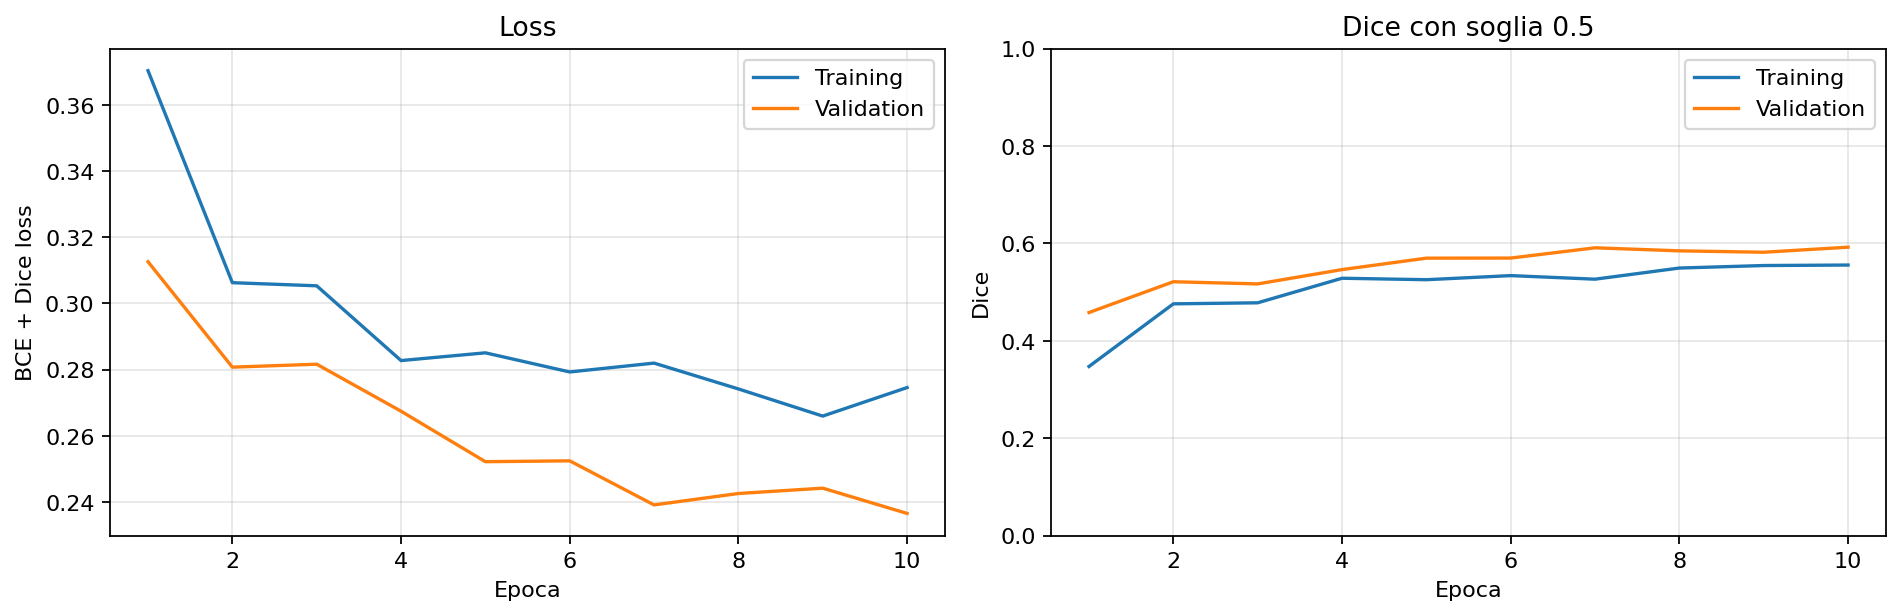
\includegraphics[width=0.72\linewidth]{../experiments/05/plots/training_curves.png}
    \caption{Experiment 5 at $1024 \times 1024$. Validation PQ, the lowest curve on
    the right, gains far more from the change of scale than Dice does.}
    \label{fig:experiment-5}
\end{figure}


\end{document}
